\chapter{Fundamentação Teórica}
\label{cap:fundamentacao}

Este capítulo apresenta os fundamentos teóricos que contextualizam a investigação.
São abordados cinco temas: fusão sensorial heterogênea, aprendizado por reforço,
inspeção em subestação de energia elétrica, sistemas robóticos e ROS/ROS2, e
navegação reativa em robótica móvel.

Convém explicitar, desde já, a relação entre esses fundamentos e o que foi
efetivamente construído. Os cinco temas delimitam o espaço de projeto no qual a
investigação se moveu e justificam as decisões tomadas; eles \emph{não} descrevem,
um a um, componentes do sistema avaliado. Em particular, a arquitetura apresentada
no Capítulo~\ref{cap:proposta} abstrai a cadeia de percepção em eventos, de modo que
a fusão sensorial da Seção~\ref{sec:fund-fusao} comparece como contexto do problema
e não como módulo implementado; e a atualização de valor discutida na
Seção~\ref{sec:fund-rl} é registrada na Seção~\ref{sec:prop-atualizacao} como nota de
projeto, por não selecionar as ações executadas pelo robô. O Capítulo~\ref{cap:conclusao}
retoma esse ajuste de escopo de forma explícita.

%% Listas convertidas em prosa em 15/11/2026: 3 de 3. O enumerate do ciclo do
%% filtro de Kalman foi MANTIDO -- e procedimento sequencial com realimentacao, nao
%% lista "Termo: explicacao".
%% Revisao estilistica em 15/11/2026. Reescritos a abertura (truismo mais
%% metadiscurso "Esta secao apresenta os conceitos essenciais"), o "aspecto
%% crucial" e o paragrafo de fechamento, que repetia o tema com adjetivos
%% elogiosos sem acrescentar conteudo. O fecho agora delimita: nenhuma tecnica
%% de fusao desta secao e implementada na tese, e a secao existe para fixar o
%% que se entende por evento sensorial.
\section{Fusão Sensorial Heterogênea}
\label{sec:fund-fusao}

Nenhuma modalidade sensorial isolada cobre as condições de uma subestação: a câmera perde o alvo sob reflexo metálico, o \ac{LiDAR} não distingue um transformador quente de um frio, o microfone não localiza o que ouve. Esta seção percorre as técnicas que combinam modalidades distintas e os limites de cada uma, para fixar o que este trabalho entende por evento sensorial.

\subsection{Conceitos Fundamentais de Fusão Sensorial}

A fusão sensorial pode ser definida como o processo de integração de dados provenientes de múltiplos sensores, com o objetivo de produzir informações mais precisas, completas e confiáveis do que seria possível utilizando cada sensor individualmente \cite{Hall1997}. Em robótica móvel, a percepção ambiental precisa ser robusta mesmo em condições adversas, como as encontradas em subestações elétricas \cite{Neto2021FiltrosRadarLidar}.

Em sistemas robóticos autônomos, a fusão sensorial busca superar as limitações inerentes a cada tipo de sensor, como limitações de alcance, sensibilidade a condições ambientais, ruído e incerteza nas medições, e interferência eletromagnética - particularmente relevante em subestações elétricas \cite{He2007EMCSubstation}.

A heterogeneidade na fusão sensorial refere-se à integração de dados provenientes de sensores de naturezas fundamentalmente distintas, como sensores visuais (câmeras \ac{RGB}), térmicos (câmeras termográficas), acústicos (microfones), de distância (\ac{LiDAR}, ultrassom), inerciais (\ac{IMU}) e químicos (sensores de gás) \cite{Alatise2020Review}. Esta abordagem multimodal permite uma percepção mais completa do ambiente, explorando as complementaridades entre diferentes modalidades sensoriais.

\subsection{Níveis de Fusão Sensorial}
A fusão sensorial pode ser realizada em diferentes níveis de abstração
\cite{Costa2018ImplementacaoFusao, Santos2023FusaoSensorial}, e o nível escolhido decide
o que se pode recuperar adiante, porque informação descartada no pré-processamento não
volta. Na \emph{fusão Z}, de baixo nível, a combinação ocorre diretamente sobre os sinais
recebidos, como intensidade de luz, distância ou temperatura: é o caso de nuvens de
pontos de múltiplos \ac{LiDAR} combinadas entre si, ou de imagens \ac{RGB} com imagens
térmicas. Na \emph{fusão F}, de nível médio, o que se combina são características já
extraídas por algum pré-processamento, como bordas, objetos detectados e velocidades, de
sorte que a fusão opera sobre vetores de características de imagem e de radar, e não
sobre as amostras brutas. Na \emph{fusão D}, de alto nível, cada sensor processa e
interpreta seus próprios dados antes da combinação, que passa a ser entre decisões: um
sensor classifica ``obstáculo'' e outro ``livre'', e a fusão resolve o conflito pela
confiança atribuída a cada um.

\begin{figure}[h]
    \centering
%% Figura refeita em 14/11/2026. A versao anterior estava errada em dois dos tres
%% niveis: o nivel medio trazia uma caixa DECISAO pendurada no sensor, que nao
%% pertence a esse nivel, e o nivel alto mostrava UM sensor seguido de QUATRO decisoes
%% soltas. As tres faixas tambem tinham estruturas diferentes entre si, de modo que a
%% figura nao deixava ver o unico ponto da taxonomia: onde, no mesmo fluxo, a fusao
%% ocorre. A versao atual usa o mesmo encadeamento nas tres faixas, variando so a
%% posicao da caixa de fusao. Reduzida de \textwidth para 0,85 por ser didatica.
    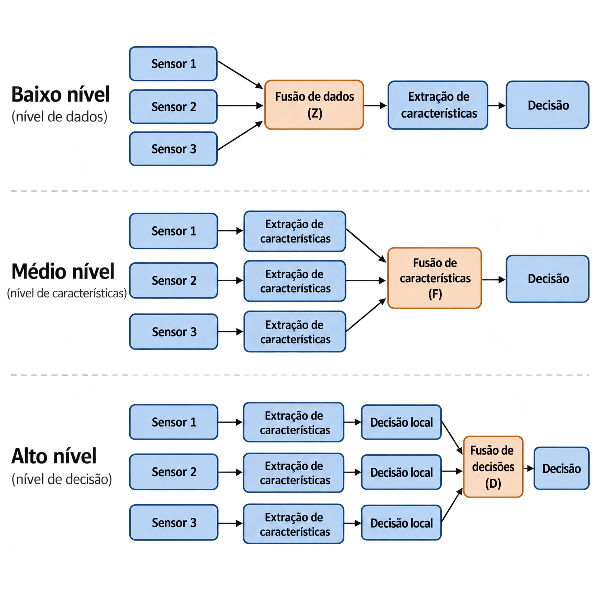
\includegraphics[width=0.85\textwidth]{figuras/fig_niveis_fusao.pdf}
    \caption{Níveis de fusão sensorial: o mesmo encadeamento de três sensores,
    variando o ponto em que a fusão ocorre --- sobre os dados brutos ($Z$), sobre as
    características extraídas ($F$) ou sobre as decisões locais de cada sensor ($D$).}
    \legend{Fonte: Elaborada pelo autor com base em \citeonline{Costa2018ImplementacaoFusao}
    e \citeonline{Santos2023FusaoSensorial}.}
    \label{fig:niveis_fusao}
\end{figure}
A \autoref{fig:niveis_fusao} ilustra os níveis de fusão sensorial.




\subsubsection{Fusão de Baixo Nível (Nível de Dados)}

A fusão de baixo nível envolve a combinação direta dos sinais provenientes dos sensores antes de qualquer extração de características ou interpretação semântica:

\begin{equation}
Z_{fusão} = f(Z_1, Z_2, ..., Z_n)
\end{equation}

Onde $Z_i$ representa os dados brutos do sensor $i$, e $f$ é a função de fusão aplicada.

Exemplos incluem combinação de nuvens de pontos de múltiplos sensores \ac{LiDAR} e fusão de imagens de diferentes espectros (\ac{RGB} + infravermelho). A principal vantagem é a preservação de toda a informação original, mas requer maior capacidade computacional e pode ser sensível a problemas de sincronização temporal e calibração espacial entre sensores \cite{Schneider2018FusaoSensores}.

\subsubsection{Fusão de Médio Nível (Nível de Características)}

A fusão de médio nível opera sobre características extraídas dos dados sensoriais brutos:

\begin{equation}
F_{fusão} = g(F_1, F_2, ..., F_n)
\end{equation}

Onde $F_i$ representa o conjunto de características extraídas do sensor $i$, e $g$ é a função de fusão aplicada às características.

Este nível oferece um bom equilíbrio entre redução de dimensionalidade (e consequentemente de carga computacional) e preservação de informação relevante \cite{Grassi2006ArquiteturaHibrida}.

\subsubsection{Fusão de Alto Nível (Nível de Decisão)}

A fusão de alto nível combina decisões ou classificações já realizadas por algoritmos específicos para cada sensor:

\begin{equation}
D_{fusão} = h(D_1, D_2, ..., D_n)
\end{equation}

Onde $D_i$ representa a decisão ou classificação baseada no sensor $i$, e $h$ é a função de fusão aplicada às decisões.

Este nível requer menor largura de banda para comunicação entre subsistemas, mas pode perder informações importantes durante o processo de decisão individual de cada sensor \cite{Ramos2012AplicacaoTecnicas}.

\subsection{Técnicas de Fusão Sensorial}

\subsubsection{Filtro de Kalman e suas Variantes}

O Filtro de Kalman é uma das técnicas mais utilizadas para fusão sensorial, especialmente para estimação de estados em sistemas dinâmicos lineares com ruído gaussiano \cite{Neto2021FiltrosRadarLidar}. 

O fluxograma que representa o Filtro de Kalman para fusão de sensores na \autoref{fig:filtro_kalman} segue as principais etapas do algoritmo de forma cíclica. 

\begin{figure}[h]
    \centering
%% Figura refeita em 14/11/2026. A versao anterior trazia "FILTRO DE KALMAN" como uma
%% caixa do fluxo, no mesmo nivel de MEDICAO e CORRECAO -- o todo desenhado como parte.
%% O ciclo tambem nao fechava, e havia duas setas sem significado (ESTADO ESTIMADO para
%% ESTADO PREVISTO contornando a PREDICAO, e CORRECAO para a caixa do filtro).
    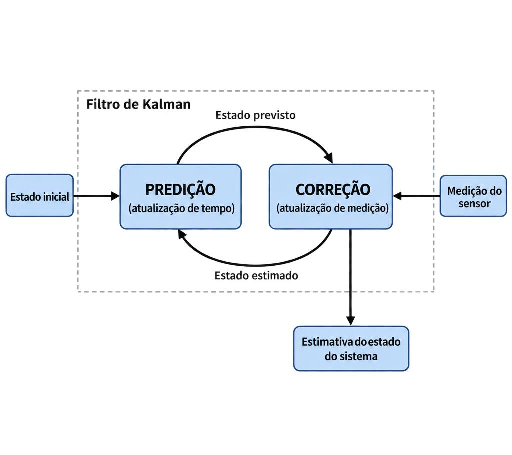
\includegraphics[width=0.8\textwidth]{figuras/fig_filtro_kalman.pdf}
    \caption{Ciclo do Filtro de Kalman: as duas fases, predição (atualização de tempo)
    e correção (atualização de medição), alternam-se indefinidamente, trocando entre si
    o estado previsto e o estado estimado. O filtro é o ciclo, não uma de suas etapas.}
    \legend{Fonte: Elaborada pelo autor.}
    \label{fig:filtro_kalman}
\end{figure}

Para cada etapa temos:

%% Reescrita em 14/11/2026, junto com a figura. A enumeracao anterior tinha tres
%% defeitos: (i) o item 1 dizia que a medicao "nao esta explicitamente rotulada" na
%% figura, o que deixou de ser verdade; (ii) o item 6 listava "Ciclo Recursivo do
%% Filtro de Kalman" como se fosse mais uma etapa, repetindo no texto o erro
%% categorico que a figura antiga cometia -- o ciclo e o conjunto, nao uma etapa; e
%% (iii) a ordem (medicao, correcao, estado estimado, predicao, estado previsto) nao
%% correspondia ao ciclo canonico de duas fases agora desenhado.
\begin{enumerate}
    \item \textbf{Predição (atualização de tempo).} Com base no modelo do sistema --- por exemplo, o modelo de movimento do robô ---, o filtro projeta o estado provável no instante seguinte, propagando também a incerteza associada ao processo. Seu resultado é o \emph{estado previsto}.

    \item \textbf{Medição do sensor.} Chega uma nova observação dos sensores (\ac{IMU}, GPS, \ac{LiDAR}, entre outros), que alimenta a etapa de correção. Ao contrário do estado previsto, ela é informação externa ao modelo.

    \item \textbf{Correção (atualização de medição).} Compara-se a medição com o estado previsto. Da comparação resulta o ganho de Kalman, que pondera quanto o filtro deve confiar na medição atual em relação à previsão. O resultado é o \emph{estado estimado}, melhor estimativa corrente das variáveis de estado: posição, velocidade e demais.

    \item \textbf{Realimentação.} O estado estimado retorna à predição, que projeta o instante seguinte, e o ciclo recomeça. Note-se que o filtro \emph{é} esse ciclo: predição e correção alternam-se indefinidamente, e não existe uma etapa separada à qual caiba o nome de filtro de Kalman.
\end{enumerate}

O Filtro de Kalman é amplamente usado em fusão sensorial para, combinar medições ruidosas e incompletas de múltiplos sensores, obter uma estimativa mais confiável do estado do sistema e também para operar de forma online, ajustando-se em tempo real à medida que novas medições chegam.


Na etapa de predição, o estado atual é estimado com base no estado anterior e no modelo do sistema:

\begin{equation}
\hat{x}_{k|k-1} = F_k\hat{x}_{k-1|k-1} + B_ku_k
\end{equation}

\begin{equation}
P_{k|k-1} = F_kP_{k-1|k-1}F_k^T + Q_k
\end{equation}

Na etapa de atualização, a estimativa é corrigida com base nas medições dos sensores:

\begin{equation}
K_k = P_{k|k-1}H_k^T(H_kP_{k|k-1}H_k^T + R_k)^{-1}
\end{equation}

\begin{equation}
\hat{x}_{k|k} = \hat{x}_{k|k-1} + K_k(z_k - H_k\hat{x}_{k|k-1})
\end{equation}

Para sistemas não-lineares, variantes como o Filtro de Kalman Estendido (\ac{EKF}) e o Filtro de Kalman Unscented (\ac{UKF}) são utilizadas \cite{Costa2018ImplementacaoFusao}.

\subsubsection{Redes Bayesianas}

As redes Bayesianas oferecem um \textit{framework} probabilístico para modelar relações causais entre variáveis, sendo particularmente úteis para fusão sensorial de alto nível \cite{Ramos2012AplicacaoTecnicas}. A probabilidade conjunta de todas as variáveis na rede é dada por:

\begin{equation}
P(X_1, X_2, ..., X_n) = \prod_{i=1}^{n} P(X_i | Pa(X_i))
\end{equation}

Onde $Pa(X_i)$ representa o conjunto de pais do nó $X_i$ no grafo.

Em fusão sensorial, as redes Bayesianas permitem integrar informações de diferentes sensores considerando suas incertezas e relações causais.

\subsubsection{Redes Neurais e Aprendizado Profundo}

Técnicas de aprendizado de máquina, especialmente redes neurais profundas, têm sido cada vez mais aplicadas para fusão sensorial \cite{Wu2022LidarFusionSurvey, Ou2024SensorFusionDRL}. Estas abordagens permitem aprender automaticamente representações e relações complexas entre diferentes modalidades sensoriais.

Arquiteturas comuns incluem Redes Neurais Convolucionais (\ac{CNN}) para processamento de dados espaciais, Redes Neurais Recorrentes (\ac{RNN}) para sequências temporais, e arquiteturas multimodais específicas para combinar diferentes tipos de dados sensoriais.

Uma arquitetura típica de fusão sensorial baseada em aprendizado profundo pode ser representada como:

\begin{equation}
F_{fusão} = f_{fusão}(f_1(X_1), f_2(X_2), ..., f_n(X_n))
\end{equation}

Onde $X_i$ representa os dados do sensor $i$, $f_i$ é a rede neural específica para processar o sensor $i$, e $f_{fusão}$ é a rede de fusão que combina as representações intermediárias.

\subsection{Desafios da Fusão em Ambientes com Interferência Eletromagnética}

A fusão sensorial em subestações elétricas enfrenta desafios específicos devido à
presença de campos eletromagnéticos intensos \cite{He2007EMCSubstation, Yan2024CombinedNav}.
O campo induz ruído e distorção nos próprios sensores eletrônicos, e os magnéticos, os
inerciais e os de comunicação sem fio são os mais suscetíveis. A intensidade e a
distribuição espacial dessa interferência variam ao longo do tempo, de modo que um
conjunto fixo de pesos entre sensores não se sustenta por toda a missão. E a degradação
não é uniforme: cada modalidade é afetada de maneira distinta, o que transfere o problema
da filtragem de um sinal para a estratégia de fusão, que precisa decidir qual leitura
desacreditar e quando. Técnicas de mitigação incluem blindagem eletromagnética, filtragem
digital e algoritmos de detecção e compensação de interferência \cite{Yan2024CombinedNav}.

\subsection{Modelos de Pesos e Bias para Relevância Sensorial}

A ponderação relativa entre sensores determina o resultado da fusão, e precisa refletir a confiabilidade, a relevância e a qualidade momentânea de cada leitura \cite{Neto2021FiltrosRadarLidar, Schneider2018FusaoSensores}.

\subsubsection{Ponderação Baseada em Covariância}

Um método comum para atribuir pesos aos sensores é baseado na matriz de covariância do erro de medição. Sensores com menor incerteza (menor covariância) recebem maior peso. Para o caso de fusão de estimativas escalares de múltiplos sensores, a estimativa ótima é dada por:

\begin{equation}
\hat{x} = \sum_{i=1}^{n} w_i x_i
\end{equation}

Onde os pesos $w_i$ são calculados como:

\begin{equation}
w_i = \frac{\sigma_i^{-2}}{\sum_{j=1}^{n} \sigma_j^{-2}}
\end{equation}

Com $\sigma_i^2$ representando a variância do erro de medição do sensor $i$.

\subsubsection{Ponderação Adaptativa Baseada em Contexto}

Em ambientes dinâmicos como subestações elétricas, a confiabilidade dos sensores pode variar em função do contexto operacional. Modelos adaptativos de ponderação consideram fatores contextuais para ajustar os pesos dos sensores em tempo real \cite{Yan2024CombinedNav}:

\begin{equation}
w_i(t) = f_w(w_i^{base}, c_1(t), c_2(t), ..., c_m(t))
\end{equation}

Onde $w_i(t)$ é o peso do sensor $i$ no instante $t$, $w_i^{base}$ é o peso base do sensor $i$, $c_j(t)$ são fatores contextuais (nível de interferência eletromagnética, iluminação, etc.), e $f_w$ é a função de adaptação dos pesos.

\subsection{Aplicações em Robótica Móvel para Inspeção}

A fusão sensorial heterogênea é particularmente relevante para robôs de inspeção em
subestações elétricas, onde diferentes tipos de sensores são necessários para detectar
diversos tipos de anomalias \cite{Lactec2022, Iberdrola2022}. A detecção de pontos
quentes combina imagem térmica com imagem visual, porque a térmica localiza o excesso de
temperatura e a visual identifica em qual componente ele está. A de descargas parciais
combina sensores acústicos, \ac{UV} e \ac{RF}, nenhum dos quais localiza a descarga
isoladamente. A navegação sob interferência eletromagnética recorre a \ac{LiDAR}, câmeras
e \ac{IMU} em conjunto, pela mesma razão que motiva a ponderação adaptativa da subseção
anterior. E a inspeção visual de corrosão, dano físico e vazamento combina as modalidades
visual, térmica e \ac{UV}, que expõem defeitos de naturezas diferentes na mesma
superfície.

Nenhuma das técnicas de fusão descritas acima é implementada nesta tese. Elas delimitam o que se entende por evento sensorial na Seção~\ref{sec:prop-sensoriamento}, onde a detecção entra no sistema já classificada por modalidade e intensidade, e o objeto de estudo passa a ser a decisão que vem depois dela.

%% Listas convertidas em prosa em 15/11/2026: 12 de 14. As duas mantidas sao
%% GLOSSARIOS DE NOTACAO imediatamente apos a definicao a que se referem (as
%% componentes da tupla do MDP e os termos da regra de atualizacao do Q). Isso e
%% convencao matematica, nao lista didatica: converter em prosa corrida piora a
%% consulta, que e a funcao delas.
%% Revisao estilistica em 15/11/2026. Reescritos a abertura e o paragrafo de
%% fechamento. O fecho anterior afirmava o "potencial do aprendizado por
%% reforco como componente fundamental" da proposta -- promessa da
%% qualificacao que a avaliacao nao sustenta. Ele agora declara o contrario,
%% que a camada principal arbitra por limiar deterministico, e diz por que.
\section{Aprendizado por Reforço}
\label{sec:fund-rl}

O Aprendizado por Reforço (\textit{Reinforcement Learning}, RL) aprende uma política por interação com o ambiente, sem exemplos rotulados de ação correta. Esta seção percorre seus elementos formais, os algoritmos relevantes para controle robótico e as razões pelas quais a camada principal desta tese não adota uma política aprendida. 

\subsection{Fundamentos do Aprendizado por Reforço}

O aprendizado por reforço é um paradigma onde um agente aprende a tomar decisões sequenciais através de interações com um ambiente, recebendo recompensas ou penalidades como feedback \cite{Sutton2018}. Diferentemente do aprendizado supervisionado ou não-supervisionado, o aprendizado por reforço foca na maximização de uma recompensa cumulativa ao longo do tempo \cite{Arulkumaran2017DeepRL}. A \autoref{fig:agente_ambiente} mostra o ciclo de interação entre o agente e o ambiente no aprendizado por reforço.

\begin{figure}[h]
    \centering
%% Figura refeita em 14/11/2026. A versao anterior omitia o ESTADO -- elemento central
%% do paradigma, listado logo abaixo e presente em toda a formalizacao do MDP -- e
%% trazia uma segunda seta do agente para o ambiente, horizontal e sem rotulo nenhum.
    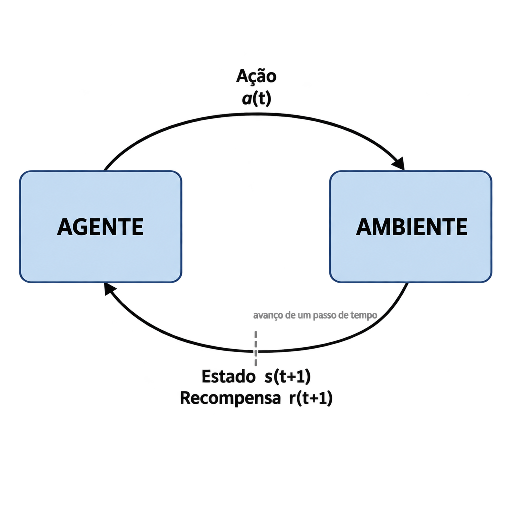
\includegraphics[width=0.8\textwidth]{figuras/fig_agente_ambiente.pdf}
    \caption{Ciclo de interação agente--ambiente no aprendizado por reforço. O agente
    emite a ação $a(t)$; o ambiente devolve o novo estado $s(t+1)$ e a recompensa
    $r(t+1)$, com o avanço de um passo de tempo assinalado sobre a seta de retorno.}
    \legend{Fonte: Elaborada pelo autor com base em \citeonline{Sutton2018}.}
    \label{fig:agente_ambiente}
\end{figure}


\subsubsection{Elementos Fundamentais}

O framework do aprendizado por reforço é composto por cinco elementos
\cite{Sutton2018}. O \emph{agente} é a entidade que decide e aprende, um robô autônomo
no caso que interessa aqui, e o \emph{ambiente} é o mundo com que ele interage, a
subestação. O \emph{estado} $s \in S$ representa a situação corrente de ambos; a
\emph{ação} $a \in A$ é a decisão do agente, capaz de alterar essa situação; e a
\emph{recompensa} $r \in \mathbb{R}$ é um escalar que informa o sucesso imediato da ação
executada. Toda a dificuldade do paradigma está nesse último elemento, porque um escalar
por passo é um canal estreito para comunicar o que se quer de um comportamento.

\subsubsection{Processo de Decisão de Markov}

O aprendizado por reforço é frequentemente formalizado como um Processo de Decisão de Markov (MDP), definido pela tupla $(S, A, P, R, \gamma)$ \cite{Puterman2014}:

\begin{itemize}
    \item $S$ é o conjunto de estados possíveis.
    \item $A$ é o conjunto de ações possíveis.
    \item $P: S \times A \times S \rightarrow [0, 1]$ é a função de transição de estados.
    \item $R: S \times A \times S \rightarrow \mathbb{R}$ é a função de recompensa.
    \item $\gamma \in [0, 1]$ é o fator de desconto, que determina a importância de recompensas futuras.
\end{itemize}

A propriedade de Markov estabelece que o próximo estado e a recompensa dependem apenas do estado atual e da ação tomada, não da história completa de estados e ações anteriores.

\subsubsection{Política e Função Valor}

O objetivo do agente é aprender uma política ótima $\pi^*: S \rightarrow A$ que maximize a recompensa cumulativa esperada. A política $\pi$ mapeia estados para ações (ou distribuições de probabilidade sobre ações) \cite{Sutton2018}.

A recompensa cumulativa descontada a partir do estado $s$ seguindo a política $\pi$ é definida como:

\begin{equation}
G_t = \sum_{k=0}^{\infty} \gamma^k R_{t+k+1}
\end{equation}

Duas funções são usadas para avaliar políticas. A \emph{função valor de estado}
$V^{\pi}$ dá o valor esperado de seguir a política $\pi$ a partir do estado $s$,

\begin{equation}
V^{\pi}(s) = \mathbb{E}_{\pi}[G_t | S_t = s]
\end{equation}

enquanto a \emph{função valor de ação} $Q^{\pi}$ dá o valor esperado de executar a ação
$a$ no estado $s$ e só então seguir $\pi$,

\begin{equation}
Q^{\pi}(s, a) = \mathbb{E}_{\pi}[G_t | S_t = s, A_t = a]
\end{equation}

distinção que importa porque é sobre a segunda, e não sobre a primeira, que se pode
decidir uma ação sem conhecer a dinâmica do ambiente.

\subsection{Algoritmo Q-Learning e Variantes}

O Q-Learning é um dos algoritmos mais fundamentais e amplamente utilizados no aprendizado por reforço, especialmente em aplicações robóticas \cite{Watkins1992}.

\subsubsection{Q-Learning Clássico}

O Q-Learning é um algoritmo livre de modelo (\textit{model-free}) que aprende diretamente a função valor ótima $Q^*$ sem necessidade de conhecer a dinâmica do ambiente \cite{Watkins1992}.

O algoritmo atualiza iterativamente a estimativa da função $Q$ usando a seguinte regra:

\begin{equation}
Q(s_t, a_t) \leftarrow Q(s_t, a_t) + \alpha [r_{t+1} + \gamma \max_{a} Q(s_{t+1}, a) - Q(s_t, a_t)]
\label{eq:fund-qlearning}
\end{equation}

Onde:
\begin{itemize}
    \item $\alpha \in (0, 1]$ é a taxa de aprendizado.
    \item $r_{t+1}$ é a recompensa recebida após executar a ação $a_t$ no estado $s_t$.
    \item $\gamma$ é o fator de desconto.
    \item $\max_{a} Q(s_{t+1}, a)$ é o valor máximo estimado para o próximo estado $s_{t+1}$.
\end{itemize}

%% Acrescentado em 15/11/2026. O capitulo ensinava a regra de atualizacao sem nomear a
%% equacao de Bellman, e a Secao 4.6 fala da "equacao de Bellman" e rotula sua equacao
%% como eq:prop-bellman. "Bellman" ocorria ZERO vezes em todo o Capitulo 2 e 3 vezes
%% nos capitulos posteriores: o leitor encontrava o nome depois do uso.
A expressão entre colchetes na Equação~\eqref{eq:fund-qlearning} é o \emph{erro de
diferença temporal}: a discrepância entre o valor estimado para o par corrente e a
estimativa revista à luz da recompensa observada e do melhor valor disponível no estado
seguinte. A regra desloca a estimativa na direção dessa discrepância, numa fração
$\alpha$ dela. O ponto fixo dessa iteração é a \emph{equação de Bellman} de otimalidade,
\begin{equation}
Q^*(s,a) = \mathbb{E}\!\left[\, r + \gamma \max_{a'} Q^*(s',a') \,\right],
\label{eq:fund-bellman}
\end{equation}
que caracteriza a função valor ótima por uma condição de consistência: o valor de um par
estado-ação é a recompensa imediata esperada mais o valor descontado do melhor que se pode
fazer em seguida. Não é uma regra de cálculo, e sim a identidade que a solução satisfaz; o
Q-Learning é um dos procedimentos que convergem para ela. Essa distinção entre a
\emph{identidade} e o \emph{procedimento} será retomada no
Capítulo~\ref{cap:proposta}, onde se discute o que significa acrescentar um termo à
atualização sem alterar a identidade que ela persegue.

Uma característica importante do Q-Learning é o dilema exploração-explotação: o agente precisa balancear entre explorar novas ações (para descobrir melhores estratégias) e explotar o conhecimento atual (para maximizar recompensas). A estratégia $\epsilon$-greedy é comumente utilizada, onde com probabilidade $\epsilon$, escolhe-se uma ação aleatória (exploração); caso contrário, escolhe-se a ação com maior valor Q (explotação).

\subsubsection{Variantes do Q-Learning}

\paragraph{SARSA}

SARSA (State-Action-Reward-State-Action) é uma variante do Q-Learning que utiliza a política atual para atualizar os valores Q \cite{Rummery1994}. A regra de atualização é:

\begin{equation}
Q(s_t, a_t) \leftarrow Q(s_t, a_t) + \alpha [r_{t+1} + \gamma Q(s_{t+1}, a_{t+1}) - Q(s_t, a_t)]
\end{equation}

A principal diferença entre Q-Learning e SARSA é que o Q-Learning é um algoritmo \textit{off-policy} (aprende a política ótima independentemente da política de exploração), enquanto SARSA é \textit{on-policy} (aprende a política que está sendo seguida).

\paragraph{Double Q-Learning}

O Double Q-Learning foi proposto para mitigar o problema de superestimação presente no Q-Learning tradicional \cite{Hasselt2010}. O algoritmo mantém duas funções valor, $Q_A$ e $Q_B$, e utiliza uma para selecionar ações e outra para avaliá-las, reduzindo o viés de superestimação.

%% Secao COMPRIMIDA e ACRESCIDA em 15/11/2026. Antes: 317 palavras sobre DQN e
%% algoritmos de politica, com figura propria, e NADA sobre moldagem de recompensa.
%% O desequilibrio era mensuravel: "DQN" ocorria 6 vezes aqui e zero nos Capitulos 4
%% a 7, enquanto `shaping' e `invariancia de politica' ocorriam ZERO aqui e 3 vezes na
%% Secao 4.7, onde esta tese declara que seu campo NAO tem a forma potencial de Ng. O
%% leitor precisava ja saber o que e essa garantia para entender o que estava sendo
%% renunciado. O DQN foi mantido em forma curta porque o Capitulo 3 depende dele (13
%% ocorrencias de DRL/DQN la), mas a figura fig_dqn saiu: ela detalhava rede alvo e
%% buffer de repeticao, que nenhum capitulo posterior usa.
\subsection{Aprendizado por Reforço Profundo}

O aprendizado por reforço profundo substitui a tabela de valor por um aproximador
paramétrico, o que o torna aplicável a espaços de estado de alta dimensão onde a tabela
seria intratável \cite{Arulkumaran2017DeepRL}. A \textit{Deep Q-Network} aprende
$Q(s,a;\theta)$ com uma rede neural em lugar de uma entrada por par estado-ação
\cite{Mnih2015}, e as duas técnicas que a tornaram treinável atacam a mesma dificuldade,
a correlação entre amostras consecutivas: a repetição de experiências treina a rede com
mini-lotes sorteados de um \textit{buffer} de transições, quebrando a ordem temporal, e a
rede alvo mantém uma segunda cópia de parâmetros atualizada apenas periodicamente, de
sorte que o alvo da regressão não se desloca a cada passo junto com a rede que o persegue.
Uma segunda família aprende a política diretamente, em vez de derivá-la de uma função
valor \cite{Sutton1999}: os métodos \textit{actor-critic} acoplam um aprendiz de política
a um de valor \cite{Konda1999}, e o \ac{PPO} limita a magnitude de cada atualização para
estabilizar o treino \cite{Schulman2017}. Nenhuma dessas famílias é empregada nesta tese,
que opera com tabela de valor discreta; elas aparecem aqui porque a literatura revisada no
Capítulo~\ref{cap:revisao} é majoritariamente construída sobre elas.

\subsection{Moldagem de Recompensa e Invariância de Política}
\label{sec:fund-shaping}

Recompensa esparsa torna o aprendizado lento: se o sinal só chega ao alcançar o objetivo,
o agente precisa encontrá-lo por exploração antes de ter o que aprender. A \emph{moldagem
de recompensa} acrescenta à recompensa original $r$ um termo $F$ que oferece sinal
intermediário, de modo que o agente aprende sobre a soma $r+F$ em vez de sobre $r$. O
expediente é antigo e eficaz, mas introduz um risco que lhe é próprio: um termo mal
escolhido pode deslocar a política ótima, premiando um comportamento que acumula $F$ sem
cumprir a tarefa --- o caso extremo é o agente que circula indefinidamente entre estados
de alto $F$ em vez de terminar.

\citeonline{ng1999} delimitaram exatamente quando esse risco não existe. O resultado é que
$F$ preserva a política ótima para \emph{qualquer} recompensa original se e somente se
tiver a forma \emph{potencial}
\begin{equation}
F(s,a,s') = \gamma\,\Phi(s') - \Phi(s),
\label{eq:fund-shaping}
\end{equation}
isto é, se for a diferença descontada de uma função $\Phi$ sobre estados. A propriedade
tem nome: \emph{invariância de política} sob transformação de recompensa. A intuição é que
um termo dessa forma se cancela ao longo de qualquer trajetória fechada, de sorte que
nenhum ciclo acumula recompensa artificial, e o que ele altera é a velocidade do
aprendizado, não o seu destino.

A distinção importa porque fixa o ônus da prova. Um termo aditivo que \emph{não} assuma a
forma da Equação~\eqref{eq:fund-shaping} --- por ser variante no tempo, por depender de
evento observado ou por somar-se diretamente ao valor em vez de entrar como diferença de
potencial --- não herda garantia alguma, e qualquer afirmação sobre a política resultante
precisa ser demonstrada caso a caso. A Seção~\ref{sec:prop-atualizacao} retoma esse
ponto para declarar o estatuto do campo formulado nesta tese, que é precisamente um termo
dessa segunda espécie.
\subsection{Aplicações em Robótica Autônoma}

O aprendizado por reforço tem sido aplicado em robótica autônoma sobretudo em percepção, navegação e manipulação \cite{Kober2013}.

\subsubsection{Navegação Autônoma}

A navegação autônoma é uma das aplicações mais relevantes do aprendizado por reforço em robótica, especialmente em ambientes dinâmicos e não estruturados como subestações elétricas \cite{Faria2002}.

Para um robô móvel, o problema de navegação pode ser formulado como um MDP em que os
estados são representações da posição, da orientação e da percepção sensorial do robô, as
ações são comandos de movimento, tipicamente velocidades linear e angular, e as
recompensas são positivas na aproximação ao objetivo e negativas em colisões e em
comportamentos indesejados. É na terceira dessas escolhas que se concentra o trabalho de
projeto, porque ela precisa codificar, num escalar, tudo o que distingue uma trajetória
aceitável de uma inaceitável.

As abordagens de aprendizado por reforço aplicadas à navegação robótica distinguem-se
pelo que supõem sobre o mapa. A navegação \emph{baseada em mapas} aprende a se deslocar
sobre uma representação do ambiente, frequentemente combinando aprendizado com técnicas
de SLAM. A navegação \emph{reativa} dispensa o mapa explícito e aprende a responder
diretamente às percepções sensoriais \cite{Zhu2017,Tai2017}.
%% Corrigido em 14/11/2026 (auditoria bibliografica): Tai2017 sustentava o item de
%% navegacao baseada em mapas, mas o proprio titulo do trabalho e "continuous control
%% of mobile robots for MAPLESS navigation" -- e a categoria oposta. A citacao foi
%% retirada daquele item (a categoria e descritiva e nao precisa de apoio pontual) e
%% passada ao item reativo, onde descreve corretamente a fonte.
A navegação \emph{hierárquica} combina as duas, com planejamento de alto nível sobre
controle reativo de baixo nível \cite{Kulkarni2016}, e é a essa terceira família que a
arquitetura desta tese se filia, com a diferença de que a camada de alto nível aqui não
é aprendida.

\subsubsection{Inspeção Autônoma}

%% Reescrito em 13/11/2026 (auditoria bibliografica): a referencia anterior desta
%% frase nao foi localizada em nenhuma base. A alegacao de aplicacao bem-sucedida de
%% aprendizado por reforco a inspecao de subestacoes foi retirada; o que a literatura
%% verificada sustenta e o uso de aprendizado em navegacao sobre observacoes fundidas,
%% em robotica movel, e nao em inspecao de subestacao em operacao.
O aprendizado por reforço tem sido aplicado a tarefas de navegação autônoma sobre observações sensoriais fundidas \cite{Ou2024SensorFusionDRL}; sua transposição para a inspeção de infraestruturas críticas como subestações elétricas permanece, em larga medida, uma direção em aberto.

Em aplicações de inspeção, o aprendizado por reforço pode ser empregado no planejamento
de trajetórias que maximizem cobertura e qualidade, na detecção e investigação de
anomalias encontradas durante a ronda, e na adaptação do comportamento a condições
ambientais variáveis. As três tarefas diferem em horizonte: a primeira é decidida antes
da missão, a segunda durante, e a terceira ao longo de missões sucessivas.

\subsection{Desafios e Limitações}

%% Reescrito em 15/11/2026. A frase abria por "Apesar de seu potencial" e terminava em
%% dois-pontos, mas o que vinha depois era um \subsubsection: os dois-pontos nao
%% anunciavam nada. As tres restricoes nomeadas sao exatamente as tres subsecoes.
A transposição do aprendizado por reforço de jogos e de ambientes de teste simulados para o robô físico esbarra em três restrições operacionais \cite{Kober2013, Arulkumaran2017DeepRL}, tratadas nas três subseções seguintes.

\subsubsection{Eficiência de Amostra}

O aprendizado por reforço frequentemente requer um grande número de interações com o
ambiente para aprender políticas eficazes, o que é impraticável em robótica real pelo
tempo e pelo desgaste envolvidos. As mitigações usuais deslocam o custo em vez de
removê-lo: treinar em simulação antes de transferir para o mundo real troca interações
reais por uma lacuna de domínio a vencer; inicializar a política com demonstrações
humanas ou de outro sistema troca-as pela qualidade do que se demonstrou; e reutilizar
conhecimento de tarefas anteriores troca-as pela semelhança entre as tarefas, que precisa
ser verdadeira.

\subsubsection{Exploração Segura}

Em robótica, a exploração aleatória pode levar a comportamentos que danificam o robô ou o
ambiente, e os métodos de exploração segura diferem em onde colocam a restrição. A
exploração guiada por incerteza a coloca na escolha da próxima ação, dirigindo-a para
onde o agente sabe menos. As restrições de segurança a colocam na formulação do problema
ou na função de recompensa, antes do aprendizado. E as formulações com risco limitado a
colocam no critério otimizado, que passa a penalizar explicitamente a cauda ruim em vez
da média. Nesta tese a restrição está em outro lugar ainda: fora da política, numa regra
de precedência que o aprendizado não pode negociar.

\subsubsection{Generalização e Transferência}

Políticas aprendidas em um ambiente ou configuração específica frequentemente não
generalizam para novos, e os três obstáculos reconhecidos são de naturezas distintas. A
transferência \textit{sim-to-real} enfrenta uma diferença sistemática entre o simulador e
o mundo. A adaptação a ambientes não vistos no treinamento enfrenta uma diferença entre
instâncias do mesmo tipo de ambiente. E a robustez a perturbações enfrenta variação
dentro de uma única instância, durante a operação. Confundir as três faz um resultado de
simulação parecer uma garantia de campo.

\subsection{Integração com Outros Paradigmas}

Para superar as limitações do aprendizado por reforço puro, abordagens híbridas que integram outros paradigmas têm sido propostas \cite{Kober2013}:

\subsubsection{Integração com Controle Clássico}

A combinação de aprendizado por reforço com controle clássico admite três arranjos, que
diferem em qual dos dois tem a palavra final. Modelos aprendidos podem alimentar
controladores clássicos, melhorando-lhes a predição sem alterar a estrutura de controle.
Controladores clássicos podem guiar a exploração durante o aprendizado, restringindo o
que o agente chega a experimentar. E arquiteturas híbridas podem reservar as tarefas
críticas de segurança ao controlador clássico e deixar à política aprendida apenas a
otimização de desempenho, que é a divisão de responsabilidade mais próxima da adotada no
Capítulo~\ref{cap:proposta}.

\subsubsection{Integração com Planejamento Simbólico}

A integração de aprendizado por reforço com planejamento simbólico atende a tarefas de
longo prazo por três vias. Hierarquias de abstração reservam o alto nível ao planejamento
simbólico e a execução ao aprendizado. Representações simbólicas facilitam transferir
conhecimento entre tarefas, porque descrevem a tarefa em termos que sobrevivem à troca de
ambiente. E conhecimento causal explícito melhora a eficiência do aprendizado e a
interpretabilidade da política resultante, que é precisamente o que falta às políticas
puramente aprendidas quando se exige certificação.

\subsection{Aplicações Específicas em Subestações Elétricas}

A literatura aponta quatro usos do aprendizado por reforço na inspeção autônoma de
subestações \cite{Ou2024SensorFusionDRL, Wei2024Advancements}: aprender políticas de
navegação que se adaptem à interferência eletromagnética variável; aprender a priorizar
equipamentos por criticidade, histórico de falhas e indicadores de anomalia; aprender a
investigar a anomalia detectada, ajustando o comportamento para coletar informação
adicional quando necessário; e ajustar a estratégia de inspeção a condições de
iluminação, clima e interferência. Os quatro supõem que a decisão a ser aprendida seja a
decisão de inspeção, e é exatamente essa suposição que esta tese não adota.

A camada principal desta tese não usa política aprendida. O arbítrio entre inspecionar e se afastar é resolvido por limiar determinístico (Capítulo~\ref{cap:proposta}), escolha que decorre de duas das limitações expostas acima, a eficiência de amostra e a opacidade da política treinada; a tabela \textit{Q} comparece no trabalho como linha de base comparativa (Seção~\ref{sec:setup-qdriven}).

\section{Inspeção em Subestação de Energia Elétrica}

As subestações de energia elétrica representam componentes críticos do sistema elétrico de potência, responsáveis pela transformação, distribuição e controle da energia elétrica. Esta seção apresenta os fundamentos teóricos relacionados às subestações elétricas, métodos de inspeção e aplicações de sistemas robóticos neste contexto.

\subsection{Fundamentos de Subestações Elétricas}
\begin{figure}[h!]
    \centering
%% Figura refeita em 14/11/2026. Na versao anterior o rotulo "Transformador de
%% potencia" aparecia DUAS vezes apontando para objetos diferentes; o rotulo
%% "Barramentos" apontava para uma interligacao em vez do barramento principal; um ramo
%% inteiro ficava sem identificacao; e o para-raios estava em serie na linha, com um
%% aterramento no meio da propria linha principal -- eletricamente, um curto.
    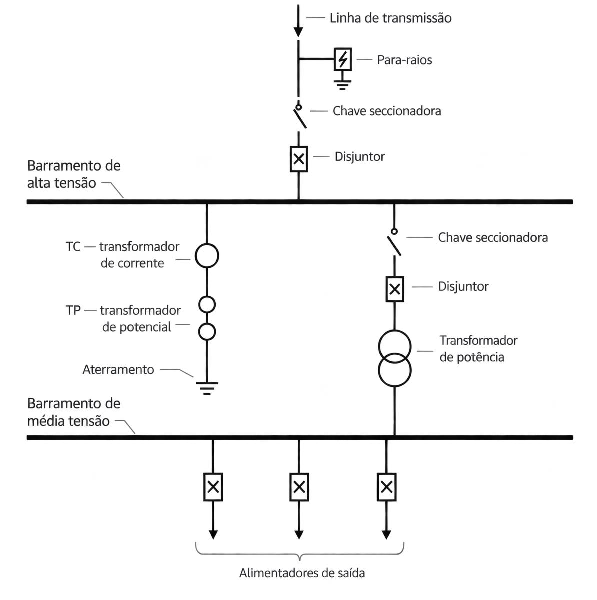
\includegraphics[width=0.8\textwidth]{figuras/fig_subestacao_tipica.pdf}
    \caption{Diagrama unifilar simplificado de uma subestação elétrica típica, da linha
    de transmissão aos alimentadores de saída, com o vão de medição (TC e TP) e o vão de
    transformação derivados do barramento de alta tensão.}
    \legend{Fonte: Adaptado de \citeonline{Muzy2012}.}
    \label{fig:subestacao_tipica}
\end{figure}

Subestações elétricas são instalações que contêm equipamentos para transmissão e distribuição de energia elétrica, além de equipamentos de proteção, medição e controle \cite{Muzy2012}. Elas desempenham funções essenciais no sistema elétrico, incluindo transformação de tensão, seccionamento de linhas, compensação de reativos e interligação de sistemas \cite{Kindermann2012}.

\subsubsection{Classificação e Componentes Principais}

As subestações podem ser classificadas segundo diversos critérios \cite{Mamede2017}:

\begin{itemize}
    \item \textbf{Quanto à função}: Elevadoras, abaixadoras, seccionadoras e de manobra.
    \item \textbf{Quanto ao nível de tensão}: Baixa tensão (até 1 kV), média tensão (1-36,2 kV), alta tensão (36,2-230 kV), extra-alta tensão (acima de 230 kV) e ultra-alta tensão (acima de 800 kV).
    \item \textbf{Quanto ao tipo de instalação}: Convencionais, abrigadas, blindadas, subterrâneas e móveis.
\end{itemize}

Os principais componentes de uma subestação incluem \cite{Frontin2013}:

\begin{itemize}
    \item \textbf{Transformadores de potência}: Responsáveis pela transformação dos níveis de tensão.
    \item \textbf{Equipamentos de manobra}: Disjuntores e chaves seccionadoras.
    \item \textbf{Transformadores de instrumentação}: TCs e TPs para medição e proteção.
    \item \textbf{Equipamentos de proteção}: Para-raios, relés e sistemas de aterramento.
    \item \textbf{Sistemas de controle e supervisão}: SCADA e dispositivos eletrônicos inteligentes (IEDs).
\end{itemize}

O arranjo de barramentos define a configuração física e elétrica da subestação, impactando sua confiabilidade, flexibilidade operativa e custo. Os principais arranjos incluem barra simples, barra principal e transferência, barra dupla, disjuntor e meio, e configuração em anel \cite{Frontin2013}.

\subsection{Normas Técnicas e Regulamentação}

As subestações elétricas são regidas por um conjunto abrangente de normas técnicas e regulamentações que visam garantir a segurança, confiabilidade e padronização das instalações \cite{ABNT2021}. No Brasil, destacam-se as normas ABNT NBR 14039 (média tensão), NBR 5410 (baixa tensão) e NBR 5419 (proteção contra descargas atmosféricas).

Internacionalmente, as normas IEC 61936-1, IEC 62271, IEC 60076 e IEC 61850 estabelecem padrões para instalações de alta tensão, equipamentos de manobra, transformadores e comunicação em subestações, respectivamente \cite{ABNT2021}.

O setor elétrico brasileiro é regulado pela ANEEL (regulação e fiscalização), ONS (operação do sistema), EPE (planejamento) e CCEE (comercialização), com os Procedimentos de Rede do ONS estabelecendo requisitos mínimos para subestações \cite{ONS2020}.

\subsection{Métodos Tradicionais de Inspeção}

A inspeção de subestações elétricas é fundamental para garantir a confiabilidade, segurança e eficiência do sistema elétrico. Tradicionalmente, estas inspeções são realizadas por técnicos especializados, seguindo procedimentos e periodicidades estabelecidos em normas e manuais de manutenção \cite{Silva2019}.

\subsubsection{Principais Métodos}

Os métodos tradicionais de inspeção incluem:

\begin{itemize}
    \item \textbf{Inspeção Visual}: Observação direta dos equipamentos para identificar vazamentos, danos físicos, conexões soltas, trincas em isoladores e outros problemas visíveis \cite{Inovarum2017}.
    
    \item \textbf{Ensaios Elétricos}: Medições de resistência de isolamento, resistência de contato, relação de transformação, fator de potência e testes funcionais de proteção \cite{Conprove2019}.
    
    \item \textbf{Análises Físico-Químicas}: Avaliação de propriedades do óleo isolante, análise de gases dissolvidos e compostos furânicos para equipamentos como transformadores e disjuntores \cite{Inovarum2017}.
    
    \item \textbf{Termografia}: Identificação de pontos de aquecimento anormal através de câmeras termográficas, indicativos de problemas como maus contatos ou sobrecargas \cite{Pixforce2024}.
    
    \item \textbf{Medição de Descargas Parciais}: Detecção de falhas incipientes em isolação elétrica através de métodos acústicos, elétricos ou UHF \cite{Frontin2013}.
\end{itemize}

\subsubsection{Limitações dos Métodos Tradicionais}

Apesar de sua eficácia, os métodos tradicionais apresentam limitações significativas \cite{GlobalGrowthInsights2024}:

\begin{itemize}
    \item \textbf{Exposição a riscos}: Os técnicos estão expostos a riscos elétricos, mecânicos e ambientais.
    \item \textbf{Necessidade de desligamento}: Muitos ensaios requerem o desligamento dos equipamentos.
    \item \textbf{Subjetividade}: A interpretação dos resultados pode variar conforme a experiência do inspetor.
    \item \textbf{Periodicidade limitada}: As inspeções são realizadas em intervalos predefinidos.
    \item \textbf{Custo elevado}: Inspeções manuais requerem mão de obra especializada.
    \item \textbf{Acesso limitado}: Alguns componentes são de difícil acesso para inspeção manual.
\end{itemize}

\subsection{Métodos Avançados e Automatizados de Inspeção}

Para superar as limitações dos métodos tradicionais, têm sido desenvolvidas técnicas avançadas e automatizadas de inspeção, que permitem monitoramento contínuo, maior segurança e detecção precoce de falhas \cite{Wei2024Advancements}.

\subsubsection{Monitoramento Online e Sistemas Integrados}

O monitoramento online permite a avaliação contínua do estado dos equipamentos sem necessidade de desligamento, utilizando sensores para gases dissolvidos em óleo, descargas parciais, temperatura, vibração e sinais acústicos \cite{Clouglobal2024}.

Sistemas de monitoramento integrados combinam diversos sensores e técnicas de análise, frequentemente utilizando comunicação baseada no padrão IEC 61850, que define protocolos e modelos de dados para automação de subestações \cite{Selinc2024}.

\subsubsection{Inspeção por Drones}

O uso de drones para inspeção de subestações oferece vantagens significativas \cite{Pixforce2023}:

\begin{itemize}
    \item Acesso a áreas de difícil alcance
    \item Redução da exposição de técnicos a riscos
    \item Inspeção rápida de grandes áreas
    \item Utilização de múltiplos sensores (visuais, térmicos, UV, LiDAR)
    \item Documentação visual detalhada
\end{itemize}

\subsubsection{Processamento Avançado de Dados}

O volume de dados gerado pelos sistemas de monitoramento e inspeção automatizada requer técnicas avançadas de processamento e análise, incluindo análise de Big Data, inteligência artificial, visão computacional, sistemas especialistas e modelos de Digital Twin \cite{Clouglobal2024}.

\subsection{Robótica para Inspeção de Subestações}

A utilização de robôs para inspeção de subestações representa uma evolução natural dos métodos automatizados, oferecendo vantagens adicionais em termos de segurança, eficiência e capacidade de inspeção \cite{Lactec2022}.

\subsubsection{Tipos de Robôs e Sensores}

Diferentes tipos de robôs têm sido desenvolvidos para inspeção de subestações \cite{GlobalGrowthInsights2024}:

\begin{itemize}
    \item \textbf{Robôs terrestres}: Com rodas, esteiras ou sistemas híbridos de locomoção.
    \item \textbf{Robôs aéreos}: Drones especializados com proteções contra interferência eletromagnética.
    \item \textbf{Robôs escaladores}: Capazes de escalar estruturas verticais.
    \item \textbf{Robôs para linhas energizadas}: Projetados para operar em linhas de transmissão energizadas.
\end{itemize}

Os robôs de inspeção são equipados com diversos sensores \cite{Lactec2022, Iberdrola2022}:

\begin{itemize}
    \item \textbf{Sistemas de visão}: Câmeras RGB, termográficas, UV, estereoscópicas e 360°.
    \item \textbf{Sensores de distância}: LiDAR, ultrassônicos e infravermelhos.
    \item \textbf{Sensores acústicos}: Para detecção de sons anormais, como descargas parciais.
    \item \textbf{Sensores de campo eletromagnético}: Para medição de campos elétricos e magnéticos.
    \item \textbf{Sensores inerciais e de posicionamento}: IMU, GPS/GNSS, RTK e sistemas indoor.
\end{itemize}

\subsubsection{Sistemas de Navegação e Processamento de Dados}

Os sistemas de navegação e controle permitem que os robôs se desloquem de forma segura e eficiente no ambiente da subestação \cite{Lactec2022, Eletrobras2024}, utilizando:

\begin{itemize}
    \item \textbf{Navegação autônoma}: SLAM, planejamento de trajetória e desvio de obstáculos.
    \item \textbf{Controle remoto}: Teleoperação e operação supervisionada.
    \item \textbf{Sistemas de comunicação}: Redes sem fio e comunicação redundante.
\end{itemize}

O processamento dos dados coletados pelos robôs pode ocorrer de forma embarcada (no próprio robô) ou em servidores centrais, utilizando técnicas como visão computacional, aprendizado de máquina e processamento de sinais para identificação de anomalias \cite{Iberdrola2022, Lactec2022}.

\subsection{Casos de Sucesso e Tendências}

Diversos projetos de robótica para inspeção de subestações têm sido implementados com sucesso \cite{Lactec2022, Iberdrola2022}, como:

\begin{itemize}
    \item \textbf{LACBOT}: Robô terrestre autônomo desenvolvido pelo Lactec no Brasil.
    \item \textbf{Antecursor I}: Robô terrestre desenvolvido pela Iberdrola na Espanha.
    \item \textbf{Pix Flight}: Sistema de inspeção baseado em drones desenvolvido no Brasil.
\end{itemize}

As principais tendências na área incluem \cite{GlobalGrowthInsights2024, Wei2024Advancements}:

\begin{itemize}
    \item Maior autonomia dos sistemas robóticos
    \item Utilização de múltiplos robôs cooperativos
    \item Implementação de algoritmos de inteligência artificial mais sofisticados
    \item Integração com modelos digitais (digital twins)
    \item Evolução para robôs capazes de realizar intervenções simples
    \item Implementação de sistemas de recarga autônoma
\end{itemize}

\subsection{Impactos na Manutenção e Operação}

A adoção de sistemas robóticos para inspeção de subestações tem potencial para transformar significativamente as práticas de manutenção e operação \cite{Wei2024Advancements, GlobalGrowthInsights2024}:

\begin{itemize}
    \item \textbf{Evolução para manutenção preditiva}: Intervenções baseadas no estado real dos equipamentos e previsão de falhas.
    \item \textbf{Aumento da confiabilidade}: Detecção precoce de anomalias, redução de falhas inesperadas e extensão da vida útil dos equipamentos.
    \item \textbf{Benefícios econômicos}: Redução de custos operacionais e de perdas por interrupção, apesar do investimento inicial significativo.
    \item \textbf{Segurança do trabalho}: Redução da exposição de trabalhadores a riscos elétricos, trabalho em altura e condições adversas.
\end{itemize}

A inspeção robótica em subestações elétricas representa um campo em rápida evolução, com potencial para superar as limitações dos métodos tradicionais e contribuir significativamente para a modernização e eficiência do setor elétrico.

%% Listas convertidas em prosa em 15/11/2026: 5 de 5. A lista dos paradigmas
%% arquiteturais foi dividida em dois paragrafos porque o proprio texto de abertura
%% dizia que a arquitetura baseada em componentes "nao figura na comparacao" por
%% estar em outro eixo -- distincao que a lista unica apagava.
%% Revisao estilistica em 15/11/2026. Reescritos a abertura e o fechamento. O
%% fecho anterior elogiava o ROS como "ecossistema maduro"; ele agora encerra
%% no determinismo de temporizacao, que e o ponto desta secao com consequencia
%% no restante do trabalho: um temporizador em tempo simulado chamando codigo
%% que consulta o relogio de parede, conforme a Secao de relogios do Cap. 4.
\section{Sistemas Robóticos e ROS/ROS2}

Um robô autônomo coordena dezenas de processos que leem sensores, estimam estado e comandam atuadores em taxas distintas, e é o \textit{middleware} que define como esses processos trocam dados e como o tempo é contado entre eles. Esta seção trata do \ac{ROS} e de sua segunda versão, sobre os quais a implementação avaliada nesta tese foi construída.

\subsection{Arquitetura de Sistemas Robóticos}

Um sistema robótico pode ser definido como um conjunto integrado de componentes de hardware e software que permitem a um robô perceber o ambiente, processar informações e executar ações \cite{Siegwart2011}. A arquitetura de software desses sistemas passou, ao longo das últimas décadas, de abordagens monolíticas para arquiteturas modulares e distribuídas \cite{Kortenkamp2016}.

\subsubsection{Componentes Fundamentais}

Os sistemas robóticos típicos são compostos por subsistemas interconectados
\cite{Siegwart2011, Kortenkamp2016}: o de percepção, que adquire e processa dados
sensoriais; o de controle, que planeja e executa ações; o de atuação, que interage
fisicamente com o ambiente; o de comunicação, que faz circular informação entre os
demais; e o de energia, que fornece e gerencia a potência disponível. O que esta tese
estuda está inteiramente no segundo, e supõe os outros quatro resolvidos.

\subsubsection{Paradigmas Arquiteturais}

A \autoref{fig:arquiteturas_roboticas} compara os três paradigmas de \emph{fluxo de
controle} propostos para organizar e integrar os componentes de software
\cite{Kortenkamp2016, Brugali2009ComponentI}, mostrando como percepção, planejamento e
atuação se conectam em cada um. A arquitetura \emph{deliberativa} segue o paradigma
\textit{Sense-Plan-Act}, adequado a ambientes estruturados e tarefas bem definidas, e
paga por isso o preço de replanejar quando o ambiente muda. A \emph{reativa} compõe
comportamentos simples que mapeiam percepção diretamente em ação \cite{Brooks1986},
respondendo rápido e sem representação global do que a cerca. A \emph{híbrida} combina as
duas, tipicamente em camadas, e é a família a que pertence a proposta do
Capítulo~\ref{cap:proposta}.

Fora desse eixo está a arquitetura \emph{baseada em componentes}, que organiza o sistema
em módulos reutilizáveis com interfaces bem definidas e fundamenta o ROS
\cite{Brugali2009ComponentI}. Ela não é uma forma de encadear percepção e ação, e por
isso não figura na comparação da figura: é ortogonal às outras três, e um sistema
deliberativo, reativo ou híbrido pode ser construído sobre ela indiferentemente.

Os principais desafios arquiteturais incluem heterogeneidade de componentes, distribuição, concorrência, requisitos de tempo real, robustez, escalabilidade e reutilização de código \cite{Kortenkamp2016, Brugali2009ComponentI}.

\begin{figure}[h]
    \centering
%% Figura refeita em 14/11/2026. A versao anterior era um infografico de apresentacao:
%% icones decorativos sem relacao com o conteudo (uma casinha em balao de fala para
%% "Arquitetura Reativa", pecas de encaixe para "Baseada em Componentes"), texto que
%% nao constava da tese ("estrutura alta"/"estrutura baixa"), ordem embaralhada em
%% relacao a lista acima e titulo interno duplicando a legenda. Sobretudo, nao mostrava
%% arquitetura alguma: eram quatro rotulos com icones, sem o encadeamento entre
%% percepcao, planejamento e atuacao, que e o que distingue os paradigmas.
    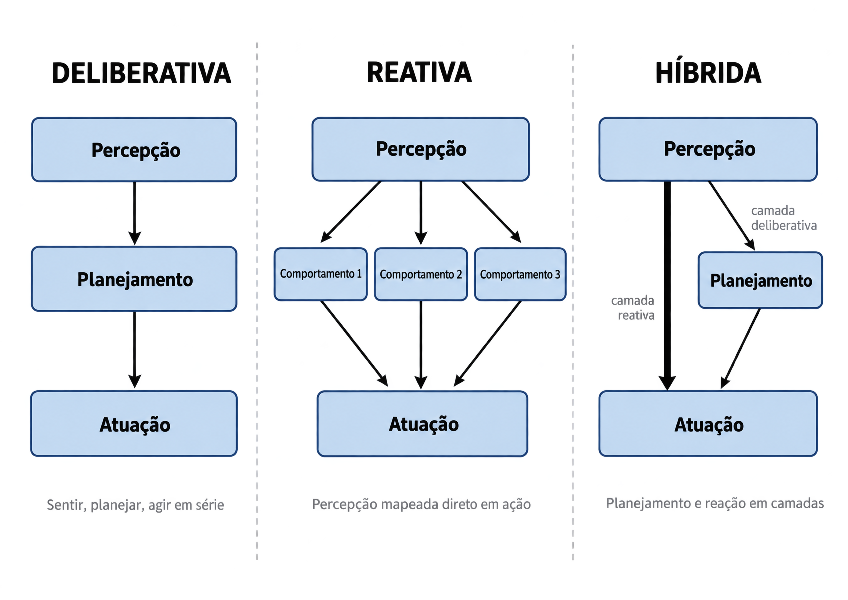
\includegraphics[width=0.8\textwidth]{figuras/fig_arquiteturas_roboticas.pdf}
    \caption{Paradigmas arquiteturais em robótica: as três colunas empregam as mesmas
    caixas --- percepção, planejamento e atuação ---, variando apenas como se conectam.
%% Corrigido em 14/11/2026: a legenda dizia que a camada reativa "alcanca a
%% atuacao sem passar pelo planejamento" e que esse e o paradigma da proposta. Nao e o
%% da implementacao: a camada reativa envia METAS ao Nav2, que continua planejando e
%% controlando, e permanece o unico produtor de /cmd_vel. O que a reacao contorna e a
%% DECISAO da patrulha sobre para onde ir, nao o planejamento do movimento.
    A via rápida em traço grosso na coluna híbrida é a camada reativa, que no esquema
    canônico alcança a atuação sem passar pelo planejamento. A arquitetura proposta no
    Capítulo~\ref{cap:proposta} segue esse paradigma em um sentido mais restrito, que
    convém fixar desde já: a camada reativa \emph{preempta a decisão} da patrulha sobre
    qual meta perseguir, mas não contorna o planejamento nem o controle de movimento ---
    ela envia metas ao Nav2, que permanece o único produtor de comandos de velocidade.}
    \legend{Fonte: Adaptado de \citeonline{Kortenkamp2016} e
    \citeonline{Brugali2009ComponentI}.}
    \label{fig:arquiteturas_roboticas}
\end{figure}


\subsection{Introdução ao ROS e ROS2}

O Robot Operating System (ROS) surgiu como uma resposta aos desafios arquiteturais dos sistemas robóticos, oferecendo um framework flexível e ferramentas para o desenvolvimento de software robótico \cite{Quigley2009}.

\subsubsection{Visão Geral do ROS}

Contrariamente ao que o nome sugere, o ROS não é um sistema operacional no sentido tradicional, mas sim um middleware que fornece serviços de comunicação, abstração de hardware, gerenciamento de pacotes e ferramentas para desenvolvimento de aplicações robóticas \cite{Quigley2009, Joseph2018}.

Os principais objetivos do ROS incluem abstração de hardware, computação distribuída, reutilização de código, ferramentas para testes e depuração, e criação de um ecossistema de software para a comunidade robótica \cite{Quigley2009}.

\subsubsection{Evolução para ROS2}

Apesar do sucesso do ROS, limitações em seu design original levaram ao desenvolvimento do ROS2, uma reimplementação completa que visa abordar essas limitações e adaptar-se às novas tendências em robótica \cite{Macenski2022}.

As motivações declaradas para o desenvolvimento do ROS2
\cite{Macenski2022, ROS2Design2024} dividem-se entre garantias que o ROS original não
dava e contextos que ele não atendia. Do primeiro grupo são o suporte a tempo real, os
mecanismos de segurança de autenticação, autorização e criptografia, a robustez em redes
não ideais e a confiabilidade exigida por aplicação industrial. Do segundo, a otimização
para sistemas embarcados de recurso limitado e o suporte nativo à coordenação de
múltiplos robôs. A primeira dessas garantias é a que importa ao Capítulo~\ref{cap:proposta},
e a Seção~\ref{sec:prop-relogios} mostra que tê-la disponível não equivale a tê-la
usada corretamente.

\subsection{Arquitetura e Componentes do ROS/ROS2}

Tanto o ROS quanto o ROS2 seguem uma arquitetura baseada em componentes, com alguns conceitos fundamentais compartilhados, embora com implementações diferentes \cite{Quigley2009, Macenski2022}.

\subsubsection{Conceitos Fundamentais}

\paragraph{Nós}

Os nós são os processos computacionais básicos no ROS/ROS2, responsáveis por realizar computações específicas \cite{Quigley2009, Joseph2018}. Em ROS, os nós são processos independentes que se comunicam através do ROS Master. Em ROS2, os nós podem ser processos independentes ou componentes dentro de um mesmo processo, com comunicação gerenciada pelo middleware DDS \cite{Macenski2022}.

\paragraph{Tópicos}

Os tópicos são canais de comunicação unidirecional que seguem o padrão publicador/assinante \cite{Quigley2009, Joseph2018}. Um nó publica mensagens em um tópico, e qualquer nó interessado pode se inscrever para receber essas mensagens. A comunicação via tópicos é assíncrona e desacoplada, adequada para transmissão contínua de dados como leituras de sensores ou estados do robô \cite{Macenski2022}.

\paragraph{Serviços e Ações}

Os serviços seguem o padrão cliente/servidor, onde um nó faz uma solicitação a outro e espera por uma resposta \cite{Quigley2009, Joseph2018}. São síncronos e adequados para operações discretas que requerem uma resposta.

As ações são uma extensão dos serviços para operações de longa duração, consistindo em uma meta, feedback durante a execução e um resultado final \cite{Joseph2018, Macenski2022}. São adequadas para tarefas como navegação ou manipulação de objetos.

\paragraph{Parâmetros e Bags}

Os parâmetros são valores de configuração que podem ser acessados e modificados pelos nós \cite{Quigley2009, Joseph2018}. Em ROS, são gerenciados pelo Parameter Server; em ROS2, pelos próprios nós.

Os bags são um formato de arquivo para armazenar e reproduzir mensagens ROS/ROS2, úteis para gravar dados durante a execução e reproduzi-los posteriormente para análise ou teste \cite{Quigley2009, Joseph2018}.

\subsubsection{Middleware e Comunicação}

Uma das principais diferenças entre ROS e ROS2 está na camada de middleware que gerencia a comunicação entre os componentes do sistema \cite{Macenski2022, ROS2Design2024}. A \autoref{fig:ros_vs_ros2} contrasta as duas arquiteturas de descoberta, separando o que é registro do que é tráfego de dados.

\paragraph{ROS Master vs. DDS}
\begin{figure}[h]
    \centering
%% Figura refeita em 14/11/2026. Na versao anterior o "Middleware DDS" aparecia como
%% hub central do painel ROS2, na mesma posicao e topologia do ROS Master a esquerda --
%% de modo que os dois paineis mostravam a MESMA arquitetura com nomes diferentes no
%% meio, apagando justamente a diferenca que a secao descreve. No painel ROS, todas as
%% ligacoes passavam pelo Master, reproduzindo o equivoco de que os dados trafegam por
%% ele. A fonte tambem nao citava nada ("documentacao oficial", sem referencia).
    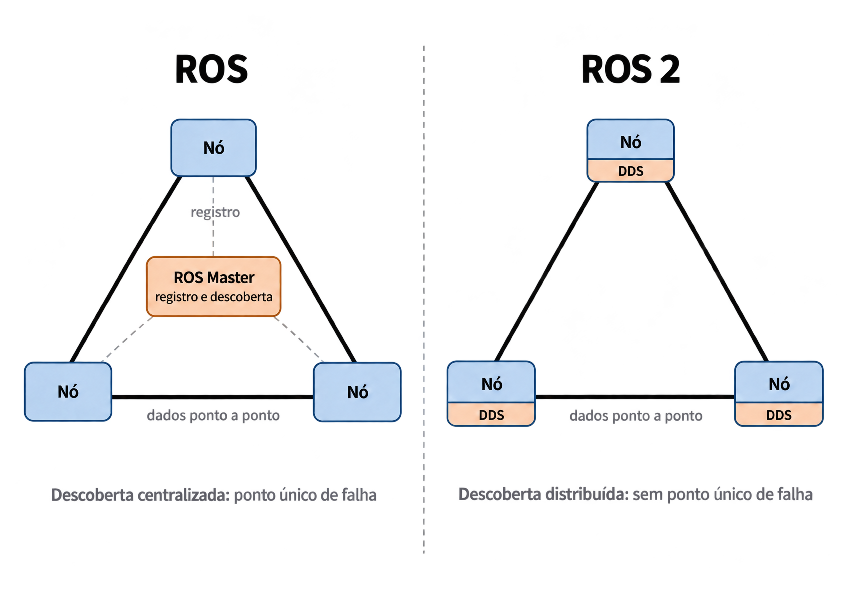
\includegraphics[width=0.8\textwidth]{figuras/fig_ros_vs_ros2.pdf}
    \caption{Arquiteturas de descoberta no ROS e no ROS~2, com os nós nas mesmas
    posições nos dois painéis. À esquerda, o registro (tracejado) é centralizado no ROS
    Master, enquanto os dados (linha cheia) trafegam ponto a ponto. À direita não há
    elemento central: o DDS reside dentro de cada nó e a descoberta é distribuída.}
    \legend{Fonte: Elaborada pelo autor com base em \citeonline{Macenski2022} e na
    documentação de projeto do ROS~2 \cite{ROS2Design2024}.}
    \label{fig:ros_vs_ros2}
\end{figure}

%% Precisado em 14/11/2026, junto com a figura: dizer que "a comunicacao e gerenciada
%% pelo ROS Master" induz a ideia de que os dados trafegam por ele, o que a figura nova
%% desmente explicitamente ao separar registro (tracejado) de dados (linha cheia).
No ROS original, é a \emph{descoberta} entre nós que é gerenciada pelo ROS Master, um serviço centralizado que mantém o registro de todos os nós, tópicos e serviços ativos \cite{Quigley2009, Joseph2018}. Concluída a negociação, os nós trocam mensagens diretamente entre si, ponto a ponto, sem que os dados passem pelo Master. Esta centralização da descoberta simplifica a implementação, mas introduz um ponto único de falha: sem o Master, nenhum nó novo encontra os demais.

O ROS2 substitui o ROS Master por uma arquitetura baseada em DDS (Data Distribution Service), um padrão aberto para comunicação publicador/assinante em sistemas distribuídos \cite{Macenski2022, ROS2Design2024}. O DDS oferece recursos avançados como descoberta distribuída, qualidade de serviço (QoS), segurança, persistência e filtragem de conteúdo.

\paragraph{Modelo de Computação}

No ROS original, cada nó é tipicamente um processo independente \cite{Quigley2009, Joseph2018}. O ROS2 introduz o conceito de composição de nós, permitindo que múltiplos nós sejam executados dentro do mesmo processo \cite{Macenski2022, ROS2Design2024}, reduzindo a sobrecarga de comunicação e permitindo compartilhamento mais eficiente de recursos.

Os executores em ROS2 gerenciam a execução de callbacks associados a tópicos, serviços, ações e timers, com diferentes tipos disponíveis (SingleThreadedExecutor, MultiThreadedExecutor, StaticSingleThreadedExecutor) para diferentes necessidades \cite{Macenski2022, ROS2Design2024}.

\subsection{Simulação e Validação}

A simulação é essencial no desenvolvimento de sistemas robóticos, permitindo testar algoritmos em ambientes virtuais antes da implementação em hardware real \cite{Siegwart2011}.

\subsubsection{Simuladores Integrados}

O ROS/ROS2 integra-se com diversos simuladores \cite{Joseph2018, Macenski2022}. O
\textbf{Gazebo} foi desenvolvido especificamente para robótica e oferece simulação de
física, de sensores, ambientes personalizáveis e extensibilidade por \textit{plugins}; é
o usado nesta tese. Webots, CoppeliaSim (V-REP), CARLA, voltado a veículos autônomos, e
Isaac Sim, da NVIDIA, também se integram ao ROS/ROS2.

\subsubsection{Ferramentas de Simulação e Teste}

O ROS/ROS2 oferece ferramentas como URDF/XACRO para descrição de robôs, RViz para visualização 3D, e rqt para interfaces gráficas \cite{Joseph2018, Macenski2022}. Para validação, integra-se com frameworks de teste unitário (GTest, pytest) e oferece ferramentas para testes de integração e integração contínua \cite{Joseph2018, Macenski2022}.

%% Subsecao NOVA em 15/11/2026, construida em torno do paragrafo que antes era a cauda
%% orfa de "Tendencias e Desenvolvimentos Futuros". O determinismo de temporizacao e a
%% unica materia desta secao que reaparece nos capitulos posteriores (15 ocorrencias de
%% tempo simulado / relogio de parede neles, contra 2 aqui), e e a fundamentacao do
%% defeito relatado na Secao 6.13. Merecia subsecao, nao um paragrafo pendurado no fim.
%% Removidas no mesmo passo as subsecoes de Integracao de Sensores e Atuadores,
%% Desenvolvimento de Aplicacoes, Aplicacoes e Casos de Uso e Tendencias: zero
%% ocorrencias de catkin, ament_cmake, setuptools, rosbag, rostopic, rosparam, tf,
%% manipulador, micro-ROS e computacao em nuvem em QUALQUER outro capitulo da tese.
\subsection{Tempo Simulado e Determinismo de Temporização}
\label{sec:fund-relogios}

Em simulação, o \ac{ROS}~2 permite que todos os nós compartilhem uma base de tempo
publicada pelo simulador, em vez do relógio do sistema operacional. Habilitado o
parâmetro correspondente, os temporizadores de cada nó passam a ser disparados por esse
tempo \emph{simulado}, de sorte que uma pausa do simulador pausa também o agendamento, e
uma simulação que corra mais devagar ou mais depressa que o tempo real não altera o
intervalo \emph{percebido} entre dois disparos \cite{Macenski2022}. É essa propriedade que
torna um experimento em simulação repetível, independentemente da carga da máquina em que
roda.

A propriedade, porém, vale para o mecanismo de agendamento, não para o código agendado.
Um temporizador pode ser disparado em tempo simulado enquanto a função que ele chama
consulta, internamente, o relógio de parede do processo --- e nada na interface sinaliza a
divergência, porque as duas leituras têm o mesmo tipo e a mesma aparência. Se essa função
compara dois instantes para decidir se um intervalo transcorreu, ela passa a medir numa
base de tempo e a ser chamada em outra, e o intervalo efetivo deixa de ser o
especificado. A Seção~\ref{sec:prop-relogios} descreve a ocorrência desse padrão na
implementação avaliada neste trabalho, e a Seção~\ref{sec:res-verificacao-relogio} mede a sua
consequência sobre os desfechos.
\section{Navegação Reativa em Robótica Móvel}

A navegação é uma capacidade fundamental para robôs móveis autônomos, permitindo que se desloquem de forma segura e eficiente em ambientes diversos. Esta seção apresenta os principais paradigmas de navegação robótica, com ênfase na navegação reativa, particularmente relevante para aplicações em ambientes dinâmicos e não estruturados como subestações elétricas.

\subsection{Paradigmas de Navegação Robótica}
A \autoref{fig:paradigmas_navegacao} mostra como a navegação robótica pode ser classificada em diferentes paradigmas, cada um com abordagens distintas para o problema de deslocamento autônomo \cite{Siegwart2011, Murphy2000}.

\begin{figure}[h]
    \centering
%% Figura refeita em 14/11/2026. A versao anterior estava errada e era redundante: a
%% coluna "Hibrida" trazia TRES caixas "Act" e NENHUMA "Plan", apagando o planejamento
%% justo onde ele define o conceito; os rotulos estavam em ingles; e o desenho repetia
%% a tricotomia da Figura~\ref{fig:arquiteturas_roboticas}, a uma secao de distancia.
%% A versao atual mostra o que e especifico de NAVEGACAO -- a mesma planta com os
%% mesmos obstaculos, variando o tracado --, de modo que as duas figuras deixam de se
%% sobrepor.
    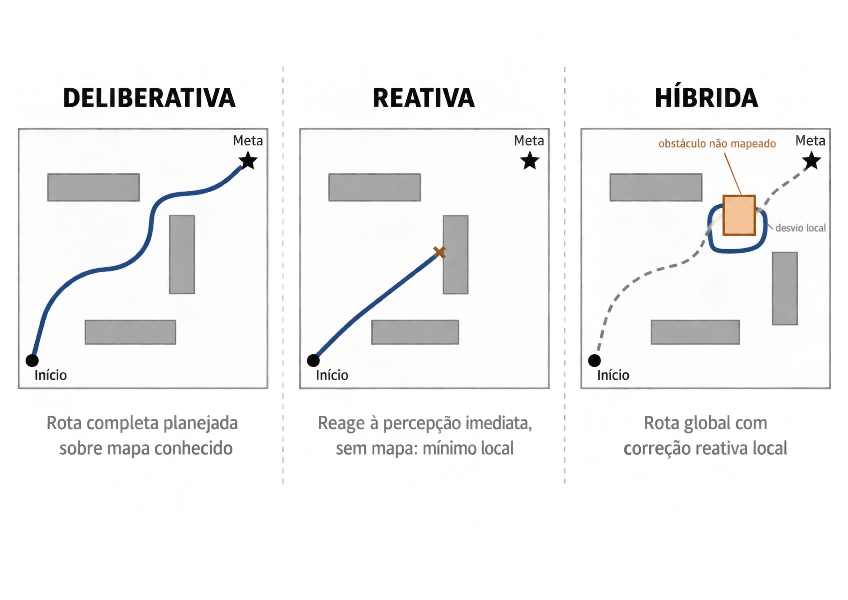
\includegraphics[width=0.8\textwidth]{figuras/fig_paradigmas_navegacao.pdf}
    \caption{Paradigmas de navegação robótica sobre a mesma planta: à esquerda, a rota
    completa planejada sobre mapa conhecido; ao centro, a reação à percepção imediata,
    que sem mapa fica retida num mínimo local antes de alcançar a meta; à direita, a
    rota global corrigida localmente ao encontrar um obstáculo não mapeado.}
    \legend{Fonte: Adaptado de \citeonline{Siegwart2011} e \citeonline{Murphy2000}.}
    \label{fig:paradigmas_navegacao}
\end{figure}


\subsubsection{Navegação Deliberativa}

A navegação deliberativa segue o paradigma Sense-Plan-Act (SPA), onde o robô percebe o ambiente, constrói um modelo interno, planeja uma trajetória completa e então a executa \cite{Murphy2000}. Suas principais características incluem:

\begin{itemize}
    \item Representação explícita do ambiente através de mapas detalhados
    \item Planejamento global de trajetórias completas
    \item Busca por soluções ótimas segundo critérios específicos
    \item Maior complexidade computacional
    \item Sensibilidade a incertezas e discrepâncias no modelo do ambiente
\end{itemize}

\subsubsection{Navegação Reativa}

Em contraste, a navegação reativa baseia-se no paradigma Sense-Act, eliminando a fase explícita de planejamento \cite{Brooks1986, Arkin1998}. O robô reage diretamente aos estímulos sensoriais, sem construir um modelo completo do ambiente. Suas características incluem:

\begin{itemize}
    \item Ausência de representação explícita do ambiente
    \item Decisões baseadas apenas na percepção imediata
    \item Baixa complexidade computacional
    \item Robustez a incertezas e mudanças no ambiente
    \item Possibilidade de soluções subótimas ou mínimos locais
\end{itemize}

\subsubsection{Navegação Híbrida}

A navegação híbrida combina elementos das abordagens deliberativa e reativa \cite{Murphy2000, Arkin1998}, tipicamente organizados em camadas:

\begin{itemize}
    \item Camada deliberativa para planejamento global e raciocínio de alto nível
    \item Camada reativa para respostas rápidas a eventos imprevistos
    \item Camada intermediária para coordenação entre as demais
\end{itemize}

Exemplos incluem a arquitetura 3T \cite{Bonasso1997}, AuRA \cite{Arkin1987} e Saphira \cite{Konolige1997}.

\subsection{Navegação Baseada em Comportamentos}

A navegação baseada em comportamentos é uma abordagem reativa que organiza o controle do robô em módulos comportamentais simples e independentes \cite{Arkin1998, Brooks1986}.

\subsubsection{Arquitetura de Subsunção}

A Arquitetura de Subsunção, proposta por Rodney Brooks \cite{Brooks1986}, organiza os comportamentos em camadas hierárquicas, onde comportamentos de nível superior podem suprimir ou inibir comportamentos de nível inferior. Suas características incluem:

\begin{itemize}
    \item Decomposição vertical em níveis de competência
    \item Incrementalidade na construção do sistema
    \item Mecanismos de supressão e inibição para coordenação
    \item Ausência de representação central do ambiente
\end{itemize}

Uma implementação típica inclui comportamentos como evitar obstáculos (nível básico), vagar, explorar, construir mapas e identificar objetos (níveis superiores) \cite{Brooks1986}.

\subsubsection{Esquemas Motores}

A abordagem de Esquemas Motores, proposta por Ronald Arkin \cite{Arkin1989}, utiliza fusão de comportamentos através de soma vetorial. Suas características incluem:

\begin{itemize}
    \item Representação vetorial de cada comportamento
    \item Fusão por soma ponderada dos vetores
    \item Pesos adaptativos para os comportamentos
    \item Paralelismo na contribuição dos comportamentos
\end{itemize}

A equação básica para a fusão de comportamentos é:

\begin{equation}
\vec{v} = \sum_{i=1}^{n} w_i \cdot \vec{v_i}
\end{equation}

onde $\vec{v}$ é o vetor resultante, $\vec{v_i}$ é o vetor gerado pelo comportamento $i$, $w_i$ é o peso associado ao comportamento $i$, e $n$ é o número total de comportamentos \cite{Arkin1998}.

\subsection{Campos Potenciais e Navegação Reativa}

O método de Campos Potenciais, introduzido por Oussama Khatib \cite{Khatib1986}, representa o ambiente como um campo de forças, onde o robô é atraído pelo objetivo e repelido por obstáculos.

\subsubsection{Princípios Fundamentais}

No método de Campos Potenciais, o robô é tratado como uma partícula sob influência de um campo potencial artificial $U(q)$, que é a soma de um potencial atrativo $U_{att}(q)$ gerado pelo objetivo e potenciais repulsivos $U_{rep}(q)$ gerados pelos obstáculos \cite{Khatib1986, Siegwart2011}:

\begin{equation}
U(q) = U_{att}(q) + U_{rep}(q)
\end{equation}

A força resultante que atua sobre o robô é o gradiente negativo do potencial total:

\begin{equation}
F(q) = -\nabla U(q) = -\nabla U_{att}(q) - \nabla U_{rep}(q) = F_{att}(q) + F_{rep}(q)
\end{equation}

O potencial atrativo é tipicamente definido como uma função quadrática da distância ao objetivo:

\begin{equation}
U_{att}(q) = \frac{1}{2} \xi \|q - q_{goal}\|^2
\end{equation}

O potencial repulsivo cresce à medida que o robô se aproxima de obstáculos:

\begin{equation}
U_{rep}(q) = 
\begin{cases}
\frac{1}{2} \eta \left(\frac{1}{\rho(q)} - \frac{1}{\rho_0}\right)^2, & \text{se } \rho(q) \leq \rho_0 \\
0, & \text{se } \rho(q) > \rho_0
\end{cases}
\end{equation}

onde $\eta$ é um fator de escala, $\rho(q)$ é a distância ao obstáculo mais próximo e $\rho_0$ é a distância de influência do obstáculo \cite{Khatib1986, Siegwart2011}.

\subsubsection{Limitações e Extensões}

Apesar de sua simplicidade e eficiência computacional, o método de Campos Potenciais apresenta algumas limitações \cite{Koren1991, Siegwart2011}:

\begin{itemize}
    \item Mínimos locais que podem "aprisionar" o robô
    \item Oscilações em passagens estreitas
    \item Dificuldades quando o objetivo está próximo a obstáculos
    \item Falta de consideração da dinâmica do robô
\end{itemize}

Diversas extensões foram propostas para superar estas limitações, incluindo Campos Potenciais Harmônicos \cite{Connolly1990}, combinação com navegação em grafo \cite{Barraquand1992}, e abordagens evolutivas \cite{Vadakkepat2000}.

\subsubsection{Aplicações em Robótica Móvel}

O método de Campos Potenciais tem sido aplicado com sucesso em diversas áreas \cite{Siegwart2011, Arkin1998}:

\begin{itemize}
    \item Robôs móveis terrestres para navegação em ambientes internos e externos
    \item Veículos aéreos não tripulados para navegação 3D
    \item Robôs manipuladores para planejamento de movimento
    \item Sistemas multi-robôs para coordenação de enxames
\end{itemize}

Em aplicações de inspeção de subestações elétricas, a navegação reativa baseada em campos potenciais oferece vantagens significativas devido à sua capacidade de responder rapidamente a obstáculos imprevistos e adaptar-se a ambientes dinâmicos \cite{Lactec2022, Iberdrola2022}.

\subsection{SLAM (Simultaneous Localization and Mapping)}

O SLAM é um problema fundamental em robótica móvel que consiste em construir um mapa do ambiente desconhecido enquanto simultaneamente se localiza neste mapa \cite{Durrant2006, Thrun2005}.

\subsubsection{O Problema do SLAM}
Os principais desafios do SLAM incluem incertezas na odometria e nas medições, associação de dados, alta dimensionalidade do espaço de estados e ambiguidade perceptual \cite{Durrant2006, Thrun2005}. A \autoref{fig:problema_slam} mostra uma visão geral do uso do SLAM na navegação.

\begin{figure}[h]
    \centering
%% Figura refeita em 14/11/2026. A versao anterior nao mostrava o problema: exibia
%% quatro setas soltas entre robo, ambiente e mapa, sem a circularidade que e a
%% dificuldade inteira do SLAM. Equiparava ainda "comandos de controle" e "odometria"
%% num unico rotulo, sendo que u sao os comandos e a odometria e a medida do
%% deslocamento resultante, com incerteza propria.
    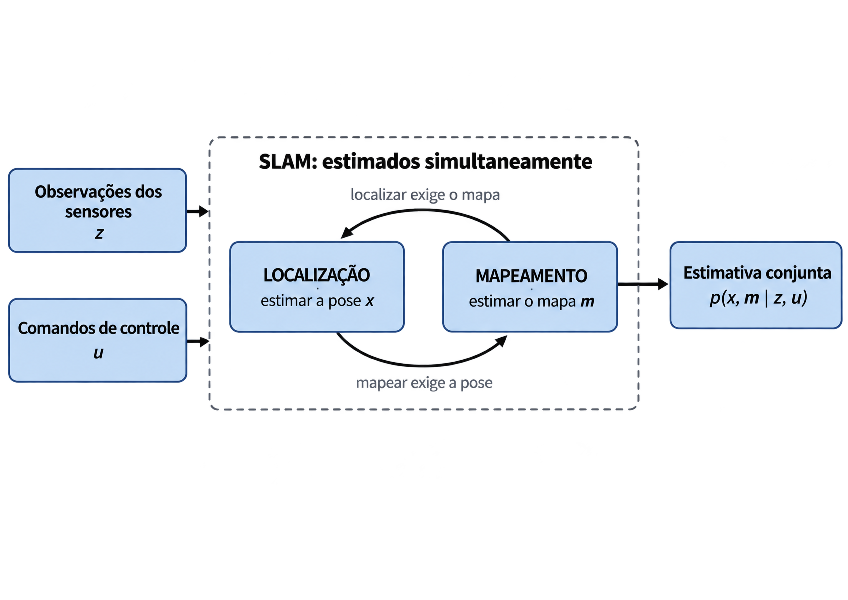
\includegraphics[width=0.8\textwidth]{figuras/fig_problema_slam.pdf}
    \caption{O problema do SLAM: localizar exige o mapa e mapear exige a pose, de modo
    que as duas estimativas são mutuamente dependentes e precisam ser resolvidas
    simultaneamente, a partir das observações $z$ e dos comandos de controle $u$.}
    \legend{Fonte: Adaptado de \citeonline{Durrant2006} e \citeonline{Thrun2005}.}
    \label{fig:problema_slam}
\end{figure}

O problema do SLAM pode ser formulado probabilisticamente como a estimação da distribuição de probabilidade conjunta \cite{Durrant2006, Thrun2005}:

\begin{equation}
p(x_{1:t}, m | z_{1:t}, u_{1:t}, x_0)
\end{equation}

onde $x_{1:t}$ são os estados do robô, $m$ é o mapa do ambiente, $z_{1:t}$ são as observações sensoriais, $u_{1:t}$ são os comandos de controle, e $x_0$ é o estado inicial.


\subsubsection{Principais Abordagens}

Diversas abordagens foram desenvolvidas para resolver o problema do SLAM \cite{Durrant2006, Thrun2005, Cadena2016}:

\begin{itemize}
    \item \textbf{SLAM Baseado em Filtros}: Utiliza técnicas como EKF-SLAM (Extended Kalman Filter) \cite{Smith1990}, UKF-SLAM (Unscented Kalman Filter) \cite{Julier2004} e FastSLAM (filtros de partículas) \cite{Montemerlo2002}.
    
    \item \textbf{SLAM Baseado em Otimização}: Formula o problema como minimização de erro, incluindo Graph-SLAM \cite{Grisetti2010} e Pose Graph Optimization.
    
    \item \textbf{SLAM Visual}: Utiliza câmeras como principal sensor, incluindo MonoSLAM \cite{Davison2007}, Stereo SLAM \cite{Paz2008} e Visual-Inertial SLAM \cite{Mourikis2007}.
    
    \item \textbf{SLAM Baseado em LiDAR}: Utiliza sensores laser, incluindo Hector SLAM \cite{Kohlbrecher2011}, Cartographer \cite{Hess2016} e LOAM \cite{Zhang2014}.
\end{itemize}

\subsubsection{Representações de Mapas}

Diferentes representações de mapas são utilizadas em SLAM \cite{Thrun2005, Cadena2016}:

\begin{itemize}
    \item Mapas de Ocupação em Grade (discretização do espaço em células) \cite{Elfes1989}
    \item Mapas de Características (pontos, linhas ou cantos distintos) \cite{Smith1990}
    \item Mapas Topológicos (grafo de locais e conexões) \cite{Kuipers1991}
    \item Mapas Semânticos (com informações sobre objetos e regiões) \cite{Kostavelis2015}
    \item Mapas 3D (nuvens de pontos, malhas ou octrees) \cite{Hornung2013}
\end{itemize}

O fechamento de loop (reconhecer quando o robô retorna a um local visitado) é o que corrige a deriva acumulada na odometria: detectado o reencontro, mapa e trajetória estimada são reajustados \cite{Durrant2006, Cadena2016}.

\subsection{Integração de Modelos 3D em Navegação}

A integração de modelos 3D em sistemas de navegação robótica representa uma tendência importante, especialmente para aplicações em ambientes complexos como subestações elétricas \cite{Hornung2013, Rusu2011}.

\subsubsection{Representações 3D para Navegação}

Diversas representações 3D são utilizadas para navegação robótica \cite{Hornung2013, Rusu2011}:

\begin{itemize}
    \item \textbf{Nuvens de Pontos}: Conjuntos de pontos 3D obtidos de sensores como LiDAR ou câmeras de profundidade.
    
    \item \textbf{Octrees}: Estruturas hierárquicas que dividem o espaço 3D recursivamente, como o OctoMap \cite{Hornung2013}.
    
    \item \textbf{Malhas Poligonais}: Representações de superfícies através de polígonos conectados.
    
    \item \textbf{Mapas de Elevação}: Representações 2.5D que armazenam a altura do terreno para cada posição (x,y).
\end{itemize}

\subsubsection{Aquisição e Processamento de Dados 3D}

A aquisição de dados 3D para navegação pode ser realizada através de \cite{Rusu2011, Hornung2013}:

\begin{itemize}
    \item Sensores LiDAR 3D ou 2D com movimento
    \item Câmeras RGB-D (como Kinect ou RealSense)
    \item Sistemas de visão estéreo
    \item Fotogrametria e Structure from Motion
\end{itemize}

O processamento destes dados envolve técnicas como registro de nuvens de pontos, filtragem, segmentação, detecção de características e reconstrução de superfícies \cite{Rusu2011}.

\subsubsection{Aplicações em Subestações Elétricas}

A integração de modelos 3D em navegação robótica para inspeção de subestações elétricas oferece diversas vantagens \cite{Lactec2022, Iberdrola2022}:

\begin{itemize}
    \item \textbf{Planejamento de Trajetória 3D}: Permite considerar a estrutura vertical das subestações, incluindo equipamentos elevados e obstáculos em diferentes alturas.
    
    \item \textbf{Localização Precisa}: Melhora a precisão da localização do robô através da correspondência com modelos 3D detalhados.
    
    \item \textbf{Detecção de Mudanças}: Permite identificar alterações na estrutura da subestação através da comparação com modelos de referência.
    
    \item \textbf{Inspeção Baseada em Modelos}: Facilita a inspeção direcionada de componentes específicos, utilizando o modelo 3D como referência.
    
    \item \textbf{Visualização e Análise}: Melhora a visualização e análise dos dados de inspeção no contexto do modelo 3D da subestação.
\end{itemize}

\subsection{Desafios e Tendências}

A navegação reativa em robótica móvel, especialmente para aplicações em subestações elétricas, enfrenta diversos desafios e apresenta tendências emergentes \cite{Cadena2016, Lactec2022, Iberdrola2022}.

\subsubsection{Desafios Atuais}

\begin{itemize}
    \item \textbf{Robustez a Interferência Eletromagnética}: Garantir o funcionamento adequado dos sensores e algoritmos de navegação em ambientes com forte interferência eletromagnética.
    
    \item \textbf{Navegação em Ambientes Complexos}: Lidar com a complexidade estrutural das subestações, incluindo equipamentos de diferentes formas e tamanhos, cabos, estruturas elevadas, etc.
    
    \item \textbf{Adaptação a Condições Variáveis}: Adaptar-se a mudanças nas condições ambientais, como iluminação, clima e configuração da subestação.
    
    \item \textbf{Segurança}: Garantir a navegação segura em ambientes de alta tensão, evitando colisões com equipamentos críticos e mantendo distâncias de segurança.
\end{itemize}

\subsubsection{Tendências Emergentes}

\begin{itemize}
    \item \textbf{Navegação Semântica}: Incorporação de informações semânticas no processo de navegação, permitindo decisões baseadas no significado e função dos objetos no ambiente.
    
    \item \textbf{Aprendizado de Navegação}: Utilização de técnicas de aprendizado de máquina para melhorar o desempenho da navegação através da experiência.
    
    \item \textbf{Navegação Colaborativa}: Coordenação entre múltiplos robôs para inspeção e navegação mais eficientes.
    
    \item \textbf{Integração com Digital Twins}: Utilização de modelos digitais detalhados das subestações para melhorar o planejamento e execução da navegação.
\end{itemize}

A navegação reativa em robótica móvel, especialmente quando integrada com técnicas de SLAM e modelos 3D, oferece uma base sólida para o desenvolvimento de sistemas robóticos autônomos capazes de realizar inspeções eficientes e seguras em subestações elétricas, contribuindo para a manutenção preventiva e a confiabilidade do sistema elétrico.

